\subsection{Lagerentnahmeentscheidung}

Die Gleichung \eqref{DP} wird in der Modellerweiterung der Lagerentnahmeentscheidung um den Parameter des Lagerbestands $y_{j}$ erweitert. In Bezug des Ausgangsproblems der Annahmeentscheidung über auftragsbezogenen Instandhaltungsprozessen ist dieser Schritt der Modellerweiterung nötig, damit ein Parameter für bereits reparierte Produkte im Modell vorhanden ist. 

Bei dieser Modellerweiterung fungiert der Parameter $y_{j}$ als Lagerbestand von Produkten $j\in\mathcal{J}$. D. h. es sind Bündel an bereits verbrauchten Ressourcen $h\in\mathcal{H}$ gemeint, die direkt den Nachfragern zur Verfügung gestellt werden. Der Parameter lässt sich als Vektor $\textbf{y}$ interpretieren, wobei die Länge des Vektors die Anzahl an Produkten $j\in\mathcal{J}$ und der sortierte Eintrag des Vektors dem Lagerbestands des Produkts $j$ entspricht. Sofern eine Anfrage über den Lagerbestand befriedigt wird, erfolgt eine Reduktion des Lagerbestand durch den Parameter $s_{jj}$. Da in dieser Modellannahme eine Anfrage nach einem Produkt $j$ auch nur mit dem Lagerbestand des Produkts $j$ angenommen werden kann, entspricht $s_{j=j}=1$ und alle anderen $s_{j\neq j}=0$. Damit lässt sich ein Vektor $\textbf{s}_j$ formen, der als Lagerentnahme für eine Anfrage nach dem Produkt $j$ dient. Weiter können die einzelnen Vektoren $s_{j}$ als Matrix $\textbf{S}$ aufgebaut werden. Die Matrix $\textbf{S}$ entspricht einer Einheitsmatrix $I_{n}\in\mathbb{R}^{n\times n}$ wobei $n=j$.

Die Gleichung \eqref{DP} lässt sich damit wie folgt formulieren:

\begin{alignat*}{2}
V(\textbf{c}, \textbf{y}, t) =\;& \sum_{j \in \mathcal{J}}p_{j}(t)\max[V(\textbf{c}, \textbf{y}, t-1), \\
& r_{j} + V(\textbf{c}-\textbf{a}_j, \textbf{y}, t-1),\\
& r_{j} + V(\textbf{c}, \textbf{y}-\textbf{s}_j, t-1)] \\
& + p_{0}(t)V(\textbf{c}, \textbf{y}, t-1)\\[10pt] 
%= \;& \sum_{j \in \mathcal{J}}p_{j}(t)V(\textbf{c}, \textbf{y}, t-1)\\
%& + \sum_{j \in \mathcal{J}}p_{j}(t)\max[r_{j} - V(\textbf{c}, \textbf{y}, t-1) + V(\textbf{c}-\textbf{a}_j, \textbf{y}, t-1),0]\\
%& +  \sum_{j \in \mathcal{J}}p_{j}(t)\max[r_{j} - V(\textbf{c}, \textbf{y}, t-1) + V(\textbf{c}, \textbf{y}-\textbf{s}_j, t-1),0]\\
%&+ p_{0}(t)V(\textbf{c}, \textbf{y}, t-1)\\[10pt] 
= \;& \sum_{j \in \mathcal{J}}p_{j}(t)V(\textbf{c}, \textbf{y}, t-1)\\
&+ \sum_{j \in \mathcal{J}}p_{j}(t)[\max[r_{j} - V(\textbf{c}, \textbf{y}, t-1)+ V(\textbf{c}-\textbf{a}_j, \textbf{y}, t-1),0]\\
&+ \max[r_{j} - V(\textbf{c}, \textbf{y}, t-1) + V(\textbf{c}, \textbf{y}-\textbf{s}_j, t-1),0]]\\
&+ p_{0}(t)V(\textbf{c}, \textbf{y}, t-1)\\
\end{alignat*}
\begin{equation}\label{stock}
\begin{alignat*}{2}
V(\textbf{c}, \textbf{y}, t) = \;& V(\textbf{c}, \textbf{y}, t-1)\\
&+ \sum_{j \in \mathcal{J}}p_{j}(t)[\max[r_{j} - V(\textbf{c}, \textbf{y}, t-1) + V(\textbf{c}-\textbf{a}_j, \textbf{y}, t-1),0]\\
&+ \max[r_{j} - V(\textbf{c}, \textbf{y}, t-1) + V(\textbf{c}, \textbf{y}-\textbf{s}_j, t-1),0]]\\
\end{alignat*}
\end{equation}

Bei der Modellformulierung $V(\textbf{c}, \textbf{y}, t)$ der \textit{Bellman'schen Funktionsgleichung} des RM mit Lagerentnahme ist der Term $ r_{j} + V(\textbf{c}, \textbf{y}-\textbf{s}_j, t-1)]$ integriert, der die Annahme mittels des Lagerbestands beschreibt. Damit ist es dem Unternehmen möglich entweder die Kapazität oder den Lagerbestand in Anspruch zu nehmen. Diese Optionen werden in dieser Arbeit durch einen weiteren Index $m$ bei dem Parameter für den Produktauftrag $j_{m}$ kenntlich gemacht. Sofern es sich um eine Auftragsannahme mittels Kapazitätsinanspruchnahme (AA) handelt, erfolgt die Annahme des Produktauftrags $j_{AA}$. Handelt es sich um eine Annahme des Auftrags mittels des Lagerentnahme (LE), dann wird der Parameter $j_{LE}$ aufgeführt.

Für die Modellerweiterung gelten die Grenzbedingungen \eqref{GB1} sowie \eqref{GB2} und es gilt zusätzlich
\begin{equation}\label{GB3}
     OP_{\textbf{c}, t}:=\left\{\begin{array}{ll} j_{AA}, & \text{für } r_{j_{AA}} - OC_{j_{AA}} \ge r_{j_{LE}} - OC_{j_{LE}}\\
         j_{LE}, & \text{für } r_{j_{AA}} - OC_{j_{AA}} < r_{j_{LE}} - OC_{j_{LE}}\end{array}\right. ,
\end{equation}
da das Unternehmen vorrangig versucht seine Kapazitäten auszulasten. Die Funktionsweise der Modellformulierung wird im nachfolgenden Beispiel verdeutlicht.
\begin{center}
$j = \{1, 2\}, \; h = \{1\}, \; r_{1} = 100, \; r_{2} = 200, \; \text{Startperiode } t=4$,
\end{center}
\[
    c_{1}=1, \;
    a_{11}=1, \;
     a_{12}=1, \;
     p_{1}(t)=\begin{pmatrix} 0.5\\ 0.5\\ 0.5\\ 0.5  \end{pmatrix}, \;
     p_{2}(t)=\begin{pmatrix} 0.1\\ 0.1\\ 0.1\\ 0.1  \end{pmatrix},
  \]
  \[
    \textbf{y}=\begin{pmatrix} 1 \\ 0 \end{pmatrix}, \;
    \textbf{s}_1=\begin{pmatrix} 1 \\ 0 \end{pmatrix}, \;
     \textbf{s}_2=\begin{pmatrix} 0 \\ 1 \end{pmatrix} \;
  \]

\begin{figure}[h!]
  \begin{center}
    \includegraphics[width=130mm]{Bilder/Beispiel3.pdf}
    \caption{Darstellung der Systemzustände des Netzwerk RM mit Möglichkeit der Lagerentnahme}  \label{B3}
    {\footnotesize \textbf{Legende:} Die Zahlen stehen für den Produktauftrag $j$, AA='Auftragsannahme', LE='Lagerentnahme', KA='Kein Auftrag'} 
  \end{center}
\end{figure}

Abbildung \ref{B3} zeigt die möglichen Systemzuständen aufgrund der vorher beschrieben Parameter. Dabei beschreibt ein Knoten weiterhin den Systemzustand. Ein Systemzustand wird durch die Zahlenfolge definiert, wobei die ersten Einträge der Zahlenfolge die Ressoucenkapazität $\textbf{c}$ entspricht. Da in diesem Beispiel nur eine Ressource vorhanden ist, beschreibt der erste Eintrag der Zahlenfolge die Ressourcenkapazität $c_{h}=1$ von $h=1$. Das Beispiel verfügt über zwei unterschiedliche Produkte $j\in\mathcal{J}$, die von den Nachfragern angefragt werden können. Somit existieren zwei Parameter für den Lagerbestand $\textbf{y}=(y_{1},y_{2})$. In dem vereinfachten Beispiel weist jedoch nur das Produkt $j=1$ einen Lagerbestand in Höhe von $y_{1}=1$ auf. Vom Produkt $j=2$ gibt es in diesem Beispiel keinen Lagerbestand. Damit entsprechen die nachfolgenden Zahlen in der Zahlenfolge des Systemzustands den möglichen Lagerbeständen $\textbf{y}$. Der letzter Wert der Zahlenfolge ist weiterhin der Zeitpunkt bzw. die Periode $t$. Der Systemzustand lässt damit wie folgt definieren: $[c_{1}\; y_{1}\; y_{2}\;t]$. Dem Unternehmen ist es möglich, unter Beachtung der vorausgehenden Parameter, entweder eine Anfrage $j_{AA}=1$ oder $j_{AA}=2$ mittels der Kapazität von $c_{1}$ anzunehmen (Auftragsannahme) oder eine Anfrage $j_{LE}=1$ mittels des Lagerbestands $y_{1}$ zu erfüllen (Lagerentnahme). Des Weiteren ist das Eintreffen keiner Anfrage zum Zeitpunkt $t$ möglich (Kein Auftrag). Damit sind die in dem Graphen aus der Abbildung \ref{B3} möglichen Systemzustände (Knoten) und Übergänge (Kanten) möglich.

\begin{table}
\begin{footnotesize}
    \caption{Ergebnistabelle für das beispielhafte Netzwerk RM mit Möglichkeit der Lagerentnahme} \label{Tab3}
    \vspace*{3mm}
    \begin{center}
\csvautotabular{data/beispiel3.csv}
      \end{center}
    \begin{center}
      {\footnotesize \textbf{Legende:} AA='Auftragsannahme', LE='Lagerentnahme', KA='Kein Auftrag'} 
      \end{center}
\end{footnotesize}
\end{table}

Die Tabelle \ref{Tab3} zeigt für das Beispiel die berechneten Erwartungswerte des noch möglichen Ertrags für jeden Systemzustand. Ebenfalls ist die optimale Politik in Form des besten Auftrags $j^*$ mit zugehörigem Ausführungsmodus $m$ aufgeführt. Dabei beschreibt hier der Ausführungsmodus die Auftragsannahme (AA), Lagerentnahme (LE) oder ob ein Auftrag keine Annahme erhält (KA). Zusätzlich ist der Wert $r_{j}-OC_{j}$ für den besten Auftrag $j^*$ je Systemzustand angegeben. Mit diesen Werten lässt sich der optimale Pfad des Beispiels ermitteln: $[2\;1\;0\;4] \rightarrow_{j_{AA}=2} [1\;1\;0\;3] \rightarrow_{j_{AA}=2} [0\;1\;0\;2] \rightarrow_{j_{LE}=1} [0\;0\;0\;1]\rightarrow_{j=0} [0\;0\;0\;0]$. Auch hier gilt weiterhin, dass der optimale Pfad abhängig der tatsächlich eintreffenden Anfragen ist. Er kann nur aber bei strategischen Entscheidung herangezogen werden.

Durch die Modellerweiterung wird gezeigt, dass ein Lagerbestand an Produkten $j\in\mathcal{J}$ den Gesamtertrag des Unternehmens erhöhen kann. Dies erfolgt jedoch aufgrund des Mechanismus, dass ein Lagerbestand eine Kapazitätserhöhung für das Unternehmen entspricht. Somit handelt es hier um eine andere Darstellung der Modellformulierung des Netzwerk RM mit verschiedenen Ausführungsmodi für die Produktanfragen $j\in\mathcal{J}$. %Eine abschließende Beurteilung der Modellerweiterung erfolgt mit Abschluss des nachfolgenden Abschnitts.

\subsection{Lagerentnahme- und Instandhaltungsentscheidung}

Im vorhergehenden Abschnitt ist die Gleichung \eqref{DP} um die Eigenschaft der Lagerentnahme erweitert. Damit sind die Entscheidungen über die Annahme eines Auftrags via Kapazitäts- oder Lagerparameter möglich. Die nachfolgende Modellerweiterung soll die Gleichung \eqref{stock} mit der Entscheidung über die gewollte Ablehnung einer Anfrage erweitern, damit die Kapazitäten für die Lagererhöhung Verwendung finden. D. h. die Kapazitäten $\textbf{c}$ werden um den Ressourcenverbrauch $\textbf{a}_{j}$ reduziert, damit der Lagerbestand $\textbf{y}$ um den Parameter für die Lagerveränderung $\textbf{s}_{j}$ für ein Produkt $j$ erhöht werden kann. In Bezug der Ausgangsproblemstellung kann das Modell insoweit verstanden werden, dass ein ein Unternehmen einen unendlichen Bestand an defekten Produkten besitzt und die Entscheidung hat, ob er seine Kapazitäten verwendet um ein defektes Produkt zu reparieren. Mit der Reparatur erfolgt die Bereitstellung eines neuwertigen Produkts auf Lager.

Die Modellformulierung für die Lagerentnahme- und Instandhaltungsentscheidung lautet wie folgt:
\begin{alignat*}{2}
V(\textbf{c}, \textbf{y}, t) =\;& \sum_{j \in \mathcal{J}}p_{j}(t)\max[V(\textbf{c}, \textbf{y}, t-1),\\
&r_{j} + V(\textbf{c}-\textbf{a}_j, \textbf{y}, t-1),\\
&r_{j} + V(\textbf{c}, \textbf{y}-\textbf{s}_j, t-1),\\
&V(\textbf{c}-\textbf{a}_j, \textbf{y}+\textbf{s}_j, t-1)]\\
&+ p_{0}(t)V(\textbf{c}, \textbf{y}, t-1) \\
\end{alignat*}
\begin{equation}\label{storage}
\begin{alignat*}{2}
= \;& V(\textbf{c}, \textbf{y}, t-1)\\
&+ \sum_{j \in \mathcal{J}}p_{j}(t)[\max[r_{j} - V(\textbf{c}, \textbf{y}, t-1) + V(\textbf{c}-\textbf{a}_j, \textbf{y}, t-1),0] \\
&+ \max[r_{j} - V(\textbf{c}, \textbf{y}, t-1) + V(\textbf{c}, \textbf{y}-\textbf{s}_j, t-1),0]\\
&+ \max[V(\textbf{c}-\textbf{a}_j, \textbf{y}+\textbf{s}_j, t-1) - V(\textbf{c}, \textbf{y}, t-1) ,0]]\\
\end{alignat*}
\end{equation}

Neben der Entscheidungen über die Auftragsannahme mittels Kapazitätsinanspruchnahme (AA) und der Lagerentnahme eines Produkts (LE) ist in dieser Modellerweiterung der Gleichung \eqref{storage} die Instandsetzung eines Produkts $j$ auf Lager $y_{j}$ möglich (IH). Dafür wird der Parameter $s_{j}$ als Lagerveränderung interpretiert. Zu beachten ist jedoch, dass bei der Entscheidung der Instandhaltung eines Produkts $j_{IH}$ kein Ertrag $r_{j_{LE}}$ erzielt wird. Des Weiteren wird ein Parameter für einen maximalen Lagerbestand $y_{j}^{max}$ für jedes Produkt $j\in\mathcal{J}$ definiert. Eine derartige Modellformulierung bringt jedoch eine spezielle Funktionsweise mit, wie nachfolgendes Beispiel verdeutlichen soll:
\begin{center}
$j = \{1, 2\}, \; h = \{1\}, \; r_{1} = 100, \; r_{2} = 200, \; \text{Startperiode } t=3$,
\end{center}
\[
    c_{1}=2, \;
    a_{11}=1, \;
     a_{12}=2, \;
     p_{1}(t)=\begin{pmatrix} 0.5\\ 0.5\\ 0.5  \end{pmatrix}, \;
     p_{2}(t)=\begin{pmatrix} 0.1\\ 0.1\\ 0.1  \end{pmatrix},
  \]
  \[
    \textbf{y}=\begin{pmatrix} 0 \\ 0 \end{pmatrix}, \;
    \textbf{y}^{max}=\begin{pmatrix} 2 \\ 1 \end{pmatrix}, \;
    \textbf{s}_1=\begin{pmatrix} 1 \\ 0 \end{pmatrix}, \;
     \textbf{s}_2=\begin{pmatrix} 0 \\ 1 \end{pmatrix} \;
  \]
\begin{figure}[h!]
  \begin{center}
    \includegraphics[width=130mm]{Bilder/Beispiel4.pdf}
    \caption{Darstellung der Systemzustände des Netzwerk RM mit Möglichkeit der Lagerentnahme und Instandhaltung}  \label{B4}
    {\footnotesize \textbf{Legende:} Die Zahlen stehen für den Produktauftrag $j$, AA='Auftragsannahme', LE='Lagerentnahme', IH='Instandhaltung', KA='Kein Auftrag'} 
  \end{center}
\end{figure}

Die Abbildung \ref{B4} zeigt alle möglichen Systemzustände und Optionen für das Beispiel. Ein Systemzustand ist definiert als Zahlenfolge $[c_{1}\; y_{1}\; y_{2}\;t]$. Es gelten die Grenzbedingungen \eqref{GB1} sowie \eqref{GB2} und
\begin{equation}\label{GB4}
     OP_{\textbf{c}, t}:=\left\{\begin{array}{lll} j_{AA}, & \text{für } r_{j_{AA}} - OC_{j_{AA}} \ge r_{j_{LE}} - OC_{j_{LE}}\\
         j_{LE}, & \text{für } r_{j_{AA}} - OC_{j_{AA}} < r_{j_{LE}} - OC_{j_{LE}}\\
         j_{IH}, & \text{sonst}\end{array}\right. .
\end{equation}
Sofern die Modellerweiterung in dieser Form definiert ist, wird niemals $OP_{\textbf{c}, t}:=j_{IH}$ gelten. Dies resultiert aus der Tatsache, dass sofern genügend Kapazitäten $\textbf{c}$ zur Produktion eines Produkts $j$ vorhanden sind, die Kapazitäten für die direkte Annahme der Produktanfrage $j$ verwendet werden. Die Entscheidung über die Produktion eines Produkts $j_{IH}$ ist für das Unternehmen nur dann sinnvoll, wenn keine Anfragen zum Zeitpunkt $t$ eintreffen und die Kapazität im weiteren Verkauf verfallen würde. Die Tabelle \ref{Tab4} zeigt die berechneten Werte für das hier aufgeführte Beispiel.
\begin{table}
\begin{footnotesize}
    \caption{Ergebnistabelle für das beispielhafte Netzwerk RM mit Möglichkeit der Lagerentnahme und Instandhaltung} \label{Tab4}
    \vspace*{3mm}
    \begin{center}
\csvautotabular{data/beispiel4.csv}
      \end{center}
    \begin{center}
      {\footnotesize \textbf{Legende:} AA='Auftragsannahme', LE='Lagerentnahme', IH='Instandhaltung', KA='Kein Auftrag'} 
      \end{center}
\end{footnotesize}
\end{table}

\subsection{Aufarbeitung von Ressourcen}

Bei der nachfolgenden Modellerweiterung wird nicht mehr von einem Produktlager ausgegangen, sondern von einem Ressourcenlager. Damit existiert für jede Ressource $h\in\mathcal{H}$ ein Lagerbestand $y_h^{res}$. Die Obergrenze des Lagerbestands wird durch den Parameter $y_{h}^{max,res}$ beschrieben. Die einzelnen Lagerbestände können als Vektor $\textbf{y}^{res}$ zusammengefasst werden. In der Modellerweiterung wird davon ausgegangen, dass Kapazitäten $c_{h}$ einer Ressource $h$ verwendet werden können, damit der Lagerbestand an Ressourcen $y_{h}$ erhöht wird. Es handelt sich damit um eine Art der Vorarbeit der Leistung. Die einzelnen Bestandteile des Produkts werden auf Lager gelegt, damit diese zu einem späteren Zeitpunkt Verwendung finden. In dieser Modellerweiterung wird davon ausgegangen, dass ein komplettes Bündel des Produkts $j$ auf Lager gelegt wird. Daher kann der Parameter $\textbf{a}_{j}$ als Ressourcenveränderung angesehen werden. Das Modell schichtet damit die Kapazität der Ressourcen $h\in\mathcal{H}$ vom Parameter $c_{h}$ zu dem Lagerbestand $y_{h}^{res}$ um. Das mathematische Modell lässt sich wie folgt beschreiben:

\begin{alignat*}{2}
V(\textbf{c}, \textbf{y}^{res}, t) =\;& \sum_{j \in \mathcal{J}}p_{j}(t)\max[V(\textbf{c}, \textbf{y}^{res}, t-1),\\
&r_{j} + V(\textbf{c}-\textbf{a}_j, \textbf{y}^{res}, t-1),\\
&r_{j} + V(\textbf{c}, \textbf{y}^{res}-\textbf{a}_j, t-1),\\
&V(\textbf{c}-\textbf{a}_j, \textbf{y}^{res}+\textbf{a}_j, t-1)]\\
&+ p_{0}(t)V(\textbf{c}, \textbf{y}^{res}, t-1) \\
\end{alignat*}
\begin{equation}\label{workup}
\begin{alignat*}{2}
= \;& V(\textbf{c}, \textbf{y}^{res}, t-1)\\
&+ \sum_{j \in \mathcal{J}}p_{j}(t)[\max[r_{j} - V(\textbf{c}, \textbf{y}^{res}, t-1) + V(\textbf{c}-\textbf{a}_j, \textbf{y}^{res}, t-1),0] \\
&+ \max[r_{j} - V(\textbf{c}, \textbf{y}^{res}, t-1) + V(\textbf{c}, \textbf{y}^{res}-\textbf{a}_j, t-1),0]\\
&+ \max[V(\textbf{c}-\textbf{a}_j, \textbf{y}^{res}+\textbf{a}_j, t-1) - V(\textbf{c}, \textbf{y}^{res}, t-1) ,0]]\\
\end{alignat*}
\end{equation}

Weiterhin gelten die Grenzbedingungen \eqref{GB1} sowie \eqref{GB2} und Gleichung \eqref{GB4}. Bei dieser Modellformulierung der Gleichung \eqref{workup} wird die Einschränkung aufgehoben, bei der die Anzahl an notwendigen Ressourcen die Entscheidung der Instandhaltung dominiert. Dies wird durch das nachfolgende Beispiel verdeutlicht:
\begin{center}
$j = \{1, 2\}, \; h = \{1\}, \; r_{1} = 100, \; r_{2} = 5000, \; \text{Startperiode } t=3$,
\end{center}
\[
    c_{1}=2, \;
    a_{11}=1, \;
     a_{12}=7, \;
     p_{1}(t)=\begin{pmatrix} 0.5\\ 0.5\\ 0.5  \end{pmatrix}, \;
     p_{2}(t)=\begin{pmatrix} 0.1\\ 0.1\\ 0.1  \end{pmatrix},
  \]
  \[
    y_{1}^{res}= 5, \;
    y_{1}^{max,res}=7
      \]
\begin{figure}[h!]
  \begin{center}
    \includegraphics[width=130mm]{Bilder/Beispiel5.pdf}
    \caption{Darstellung der Systemzustände des Netzwerk RM mit Möglichkeit der Aufarbeitung}  \label{B5}
    {\footnotesize \textbf{Legende:} Die Zahlen stehen für den Produktauftrag $j$, AA='Auftragsannahme', LE='Lagerentnahme', IH='Instandhaltung', KA='Kein Auftrag'} 
  \end{center}
\end{figure}

Abbildung \ref{B5} zeigt alle Übergänge der Systemzustände für das aufgeführte Beispiel. Die Systemzustände sind beschrieben als Zahlenfolge $[c_{1}\; y_{1}^{res}\;t]$, da bei diesem Beispiel nur eine Ressource $h$ existiert. Für die Ressource $h=1$ beträgt die Kapazität $c_{1}=2$ und der Lagerbestand $y_{1}^{res}=5$. Als Obergrenze für den Lagerbestand wird $y_{1}^{max,res}=7$ festgelegt. Aufgrund der Ressourcenveränderungsparameter $\textbf{a}_{j}$ für jedes Produkt $j\in\mathcal{J}$ gibt es die Entscheidungsmöglichkeit Auftragsannahme (AA), Lagerentnahme (LE) sowie Instandhaltung aufgrund von Aufarbeitung (IH) für jedes Produkt $j\in\mathcal{J}$. Weiterhin ist die Option zu jedem Systemzustand möglich, dass keine Anfrage eintrifft und der Wechsel in die nächste Periode ohne Kapazitäts- oder Lagerreduktion erfolgt.

Aufgrund der der Restriktionen der Kapazität $c_{1}$ und des Lagerbestands $y_{1}^{res}$ sind nicht alle möglichen Entscheidungsalternativen zu jedem Systemzustand möglich. Beispielsweise ist im Systemzustand $[2\;5\;3]$ die AA, LE sowie IH des Produkts $j=2$ nicht möglich. Jedoch kann in diesem Systemzustand die Annahme einer Anfrage nach Produkt $j=1$ erfolgen, entweder durch Kapazitäts- oder Lagerreduktion. Um eine Anfrage nach Produkt $j=2$ akzeptieren zu können, werden aufgrund des Parameters $a_{12}$ genau 7 Einheiten von der Ressource $h=1$ benötigt. Entweder müssen genügen Kapazitäten vorhanden sein, was jedoch im Beispiel nicht gegeben ist, oder der Lagerbestand $y_{1}^{res}$ muss auf 7 Einheiten der Ressource $h=1$ erhöht werden. Sofern die Erträge $r_{1}=100$ und $r_{2}=5000$ für das Beispiel angenommen sind, erhalten wir die berechneten Werte der Tabelle \ref{Tab5}.
\begin{table}
\begin{footnotesize}
    \caption{Ergebnistabelle für das beispielhafte Netzwerk RM mit Möglichkeit der Aufarbeitung} \label{Tab5}
    \vspace*{3mm}
        \begin{center}
\csvautotabular{data/beispiel5.csv}
      \end{center}
    \begin{center}
      {\footnotesize \textbf{Legende:} AA='Auftragsannahme', LE='Lagerentnahme', IH='Instandhaltung', KA='Kein Auftrag'} 
      \end{center}
\end{footnotesize}
\end{table}

Ist der Ertrag $r_{j}$ eines Produkts $j\in\mathcal{J}$ ausreichend groß bei gegebener Eintrittswahrscheinlichkeit $p_{j}(t)$ zum Zeitpunkt $t$, dann erfolgt in dem Modell der Gleichung \eqref{workup} eine Überführung der Ressourcenkapazität $c_{h}$ hin zu dem Lagerbestand $y_{h}^{res}$, sofern dies eine andere Ressourceninanspruchnahme $a_{j}$ ermöglicht. Das Beispiel zeigt eine solche optimale Politik.

Für den anfänglichen Systemzustand $[2\;5\;3]$ existieren die Systemübergänge $j_{LE}$, $j_{IH}$ und $j_{AA}$ für Anfragen nach Produkt $j=1$. Außerdem ist das Eintreffen keiner Anfrage möglich. Damit lässt sich in diesem Systemzustand ein Ertrag $r_{j}=100$ generieren. Mit der Entscheidung $j_{LE}=1$ gelangt das System zum Zustand $[2\;4\;2]$, da für eine Annahme einer Anfrage nach Produkt $j=1$ der Lagerbestand $y_{1}^{res}$ reduziert wird. Sofern die Entscheidung $j_{AA}=1$ eintrifft, gelangt das System durch Inanspruchnahme der Kapazität $c_{1}$ zum Zustand $[1\;5\;2]$. Außerdem ist der Systemwechsel zum Zustand $[1\;6\;2]$ durch $j_{IH}=1$ möglich. Aufgrund der berechneten OK ist unter Beachtung der Parameter ein Systemwechsel durch die Instandhaltung optimal (Vgl. Tabelle \ref{Tab5}). Abbildung \ref{B5} zeigt diesen und alle anderen optimalen Politiken für jeden Systemzustand. Daraus lässt dich die beste Pfad ermitteln:  $[2\;5\;3] \rightarrow_{j_{IH}=1} [1\;6\;2] \rightarrow_{j_{IH}=1} [0\;7\;1] \rightarrow_{j_{LE}=2} [0\;0\;0]$.

Es ist damit gezeigt, dass die Kapazität $c_{1}$ der Ressource $h=1$ durch den Ausführungsparameter $a_{1}$ des Produkts $j$ verwendet wird, damit der Lagerbestand $y_{1}^{res}$ jener Ressource $h=1$ erhöht wird. Damit ist zu einem späteren Zeitpunkt $t$ die Annahme der Anfrage nach Produkt $j=2$ durch die Lagerentnahme (LE) des Lagerbestands $y_{1}^{res}$ der Ressource $h=1$ möglich. Damit ist ein Gesamtertrag von $5000$ GE generiert. 

\subsection{Erneuerung von Ressourcen innerhalb des Buchungshorizonts}

Wie die vergangenen Modellerweiterungen zeigen, erfolgt mit den bisherigen Modellerweiterung eine Umschichtung der Kapazitäten des Netzwerks hin zu den Lagerbestand $\textbf{y}$ bzw. $\textbf{y}^{res}$. Sofern es sich um ein Ressourcenlager $\textbf{y}^{res}$ handelt, werden die notwendigen Kapazitäten $c_{h}$ der Ressourcen $h\in\mathcal{H}$ für ein Produkt $j$ mit niedrigem Ertrag auf den Lagerbestandsparameter $\textbf{y}^{res}$ umverteilt, damit die Akzeptanz eine nachfolgende Anfrage nach einem anderweitigen Produkt $j\in\mathcal{J}$ mit höherem Ertrag $r_{j}$ über den Lagerparameter $\textbf{y}^{res}$ erfolgen kann. %Damit ist gezeigt, dass mithilfe der Modellerweiterung der \textit{Bellman'schen Funktionsgleichung} für das Netzwerk RM die optimale Politik ist, Anfragen mit niedrigem Ertrag zugunsten zukünftiger Anfragen mit höherem Ertrag abzulehnen.
Mit der Umverteilung zum Lagerbestand $\textbf{y}^{res}$ erfolgt eine Kapazitätserhöhung der notwendigen Ressourcen $h\in\mathcal{H}$ für die Produktanfrage $j$ mit hohen Ertrag $r_j$ einher.

Wie im vorherigen Abschnitt gezeigt, müssen jedoch gewisse Rahmenbedingungen für eine Ablehnung von Produktanfragen $j\in\mathcal{J}$ mit niedrigem Ertrag gegeben sein. Die Kapazitäten $\textbf{c}$ des Netzwerks müssen einerseits ausreichend groß sein, damit Anfragen nach dem Produkt $j$ mit niedrigem Ertrag $r_{j}$ abgelehnt und auf das Lager $\textbf{y}^{res}$ umverteilt werden können, aber anderseits niedrigen als der notwendige Bedarf $\textbf{a}_{j}$ für das Produkt $j$ mit höherem Ertrag. Zusätzlich muss die Differenz zwischen den vorhanden Kapazitäten $\textbf{c}$ und der notwendigen Kapazitäten $\textbf{a}_{j}$ für die Produktanfrage $j$ mit hohem Ertrag auf dem Lager $\textbf{y}^{res}$ vorhanden sein. Wären ausreichend Kapazitäten $\textbf{c}$ für beide Arten der Produktanfragen $j\in\mathcal{J}$ möglich, dann wäre eine Umverteilung auf das Lager aufgrund der Gleichung \eqref{GB4} unnötig. Die notwendigen Kapazitäten $c_{h}$ der Ressourcen $h\in\mathcal{H}$ würden direkt für die Anfrage nach dem Produkt $j$ mit hohem Ertrag Verwendung finden und eingeplant. Die optimale Politik wäre das Produkt $j$ mit hohem Ertrag $r_{j}$ frühzeitig einzuplanen, sofern Anfragen für das Produkt unter Beachtung der Wahrscheinlichkeiten $p_{j}(t)$ zu den Zeitpunkten $t\in T$ eintreffen. Anders formuliert, die Option der Annahme einer Anfrage nach dem Produkt $j$ mit hohem Ertrag wäre im Systemzustand mit ausreichendem Kapazitäten $c_{h}$ zum Zeitpunkt $t$ möglich und, sofern der Ertrag aufgrund der OK des Netzwerks nicht zu stark beeinflussen wird, optimal.

Die Aufhebung der vorhergehenden Restriktion erfolgt durch das Einführen von regenerativen Ressourcen $h\in\mathcal{H}$ innerhalb des Buchungshorizonts $T$. Erst durch die Modellerweiterung der regenerativen Ressourcen $h\in\mathcal{H}$ erhält die Modellformulierung unter Beachtung einer Lagerhaltung von Ressourcen $\textbf{y}^{res}$ innhalb des Buchungshorizonts $T$ eine Sinnhaftigkeit. Für die Modellerweiterung wird der Parameter $\tilde{t}\in\tilde{T}$ eingeführt, wobei $\tilde{T}\subset T$ gilt. Der Parameter $\tilde{t}$ zeigt den Zeitpunkt der Regeneration der Ressourcen $h\in\mathcal{H}$ an. Durch die Regeneration erhöht sich der Wert des Kapazitätsparameters auf $\textbf{c}^{max}$. Die \textit{Bellman'schen Funktionsgleichung} für ein Netzwerk RM mit regenerativen Ressourcen innerhalb des Buchungshorizonts wird wie folgt definiert:

\begin{equation}\label{reg}
     V^{reg}(\textbf{c}, \textbf{y}^{res}, t)=\left\{\begin{array}{ll} V(\textbf{c}, \textbf{y}^{res}, t), & \forall t\neq\tilde{t}\\
         V(\textbf{c}^{max}, \textbf{y}^{res}, t), &\forall t=\tilde{t}\end{array}\right. .
\end{equation}

Es gelten weiterhin Gleichungen \eqref{GB1}, \eqref{GB2} und \eqref{GB4}. Dabei erfolgt die Ermittlung der Erwartungswerte aus der Gleichung \eqref{reg} abhängig des betrachteten Zeitpunkts $t$. Die Berechnung des Erwartungswerts $V(\textbf{c}, \textbf{y}^{res}, t)$ $\forall t\neq\tilde{t}$ erfolgt wie in Gleichung \eqref{workup} und die Berechnung des Erwartungswerts $V(\textbf{c}^{max}, \textbf{y}^{res}, t)$ $\forall t=\tilde{t}$ wie nachfolgende Gleichung zeigt:
\begin{alignat*}{2}
 V(\textbf{c}^{max}, \textbf{y}^{res}, t) = \;& V(\textbf{c}^{max}, \textbf{y}^{res}, t-1)\\
&+ \sum_{j \in \mathcal{J}}p_{j}(t)[\max[r_{j} - V(\textbf{c}^{max}, \textbf{y}^{res}, t-1)\\
&+ V(\textbf{c}^{max}-\textbf{a}_j, \textbf{y}^{res}, t-1),0] \\
&+ \max[r_{j} - V(\textbf{c}^{max}, \textbf{y}^{res}, t-1) + V(\textbf{c}^{max}, \textbf{y}^{res}-\textbf{a}_j, t-1),0]\\
&+ \max[V(\textbf{c}^{max}-\textbf{a}_j, \textbf{y}^{res}+\textbf{a}_j, t-1) - V(\textbf{c}^{max}, \textbf{y}^{res}, t-1) ,0]]\\
\end{alignat*}

Die Funktionsweise des Modells soll an einem Beispiel verdeutlicht werden:
\begin{center}
$j = \{1, 2\}, \; h = \{1\}, \; r_{1} = 100, \; r_{2} = 5000, \; \text{Startperiode } t=4, \; \tilde{t}=\{2\} $,
\end{center}
\[
    c_{1}=1, \;
    a_{11}=1, \;
     a_{12}=2, \;
     p_{1}(t)=\begin{pmatrix} 0.5\\ 0.5\\ 0.5\\ 0.5  \end{pmatrix}, \;
     p_{2}(t)=\begin{pmatrix} 0.1\\ 0.1\\ 0.1\\ 0.1  \end{pmatrix},
  \]
  \[
    y_{1}^{res}= 0, \;
    y_{1}^{max,res}=2
      \]
      
Es existieren zwei Produkte $j\in\mathcal{J}$ und eine Ressource $h\in\mathcal{H}$. Sofern eine Anfrage nach dem Produkt $j=1$ akzeptiert wird, generiert sich ein Ertrag in Höhe von $r_1=100$ GE. Bei Akzeptanz einer Produktanfrage $j=2$ erzielt das Unternehmen einen Ertrag von $r_1=5000$ GE. Beide Produktanfragen benötigen die Ressource $h=1$, wobei die Kapazität der Ressource bei $c_1=1$ liegt. Ein Anfrage nach Produkt $j=1$ benötigt $a_{11}=1$ Kapazitäten und eine Anfrage nach Produkt $j=1$ benötigt $a_{12}=2$. Der Buchungshorizont entspricht $T=4$ Perioden und zum Zeitpunkt $\tilde{t}=2$ erfolgt eine Regeneration der Ressourcen. Die Wahrscheinlichkeit des Eintreffens einer Anfragen zum Zeitpunkt $t$ entspricht $ p_{1}(t)=(0.5, 0.5, 0.5, 0.5)$ bzw. $ p_{2}(t)=(0.1, 0.1, 0.1, 0.1)$. Die Lagerkapazität $y_1^{max,res}$ ist auf 2 Einheiten beschränkt und es existiert zur Starperiode $t=4$ kein Anfangsbestand ($y_1^{res}=0$). Abbildung \ref{B6} zeigt alle möglichen Systemzustände mit den einzelnen Übergängen für das Beispiel. 

\begin{figure}[h!]
  \begin{center}
    \includegraphics[width=140mm]{Bilder/Beispiel6.pdf}
    \caption{Darstellung der Systemzustände des Netzwerk RM mit regenerativen Ressourcen}  \label{B6}
    {\footnotesize \textbf{Legende:} Die Zahlen stehen für den Produktauftrag $j$, AA='Auftragsannahme', LE='Lagerentnahme', IH='Instandhaltung', KA='Kein Auftrag', $\cdots$='Anfrage ablehnen'} 
  \end{center}
\end{figure}

Ein Systemzustand im vorausgehenden Beispiel ist definiert als Zahlenfolge $[c_1\;y^{res}_1$ $t]$. Zu beachten ist, dass in diesem Netzwerk zum Zeitpunkt $t=2$ die Ressourcen erneuert sind und dementsprechend für die betreffenden Systemzustände die Zahlenfolge $[c_1^{max}\;y^{res}_1\;2]$ gilt. Wird das Gesamtnetzwerks in Abbildung \ref{B6} betrachtet, dann ergibt sich der beste Pfad $[1\;0\;4] \rightarrow_{j_{IH}=1} [0\;1\;3] \rightarrow_{KA} [1\;1\;2] \rightarrow_{j_{IH}=1} [0\;2\;1] \rightarrow_{j_{LE}=2} [0\;0\;0]$ mit einem Gesamtertrag in Höhe von $5000$ GE. Damit ist für das hier betrachtete Netzwerk die Instandhaltung (IH) der Ressource $h=1$ optimal, damit eine Anfrage nach einem Produkt $j=2$ akzeptiert werden kann. Des Weiteren ist unter diesen Bedingungen im Systemzustand $[1\;0\;4]$ die Ablehnung der Anfrage nach einem Produkt $j=1$ die beste Politik, sofern nur diese Anfrage zum Zeitpunkt $t=4$ eintrifft. Durch diese Entscheidung gelangt das Netzwerk zum Systemzustand $[1\;0\;3]$, bei dem in weiteren Verlauf das Erreichen des Systemzustands $[1\;1\;2]$ möglich ist, bei dem die Kapazitäten regeneriert sind und der Lagerbestand $y_1^{res}$ eine Einheit der Ressource $h=1$ beinhaltet. Von diesem Systemzustand ist ein weiterer Verlauf möglich, bei dem die Anfrage nach einem Produkt $j=2$ möglich ist.

Wird im Gegensatz im Systemzustand $[1\;0\;4]$ die Anfrage nach dem Produkt $j=1$ angenommen, dann gelangt das Netzwerk in den Systemzustand $[0\;0\;3]$ und erzielt einen Ertrag in Höhe von 100 GE. Vom Systemzustand $[0\;0\;3]$ ist keine Akzeptanz mehr möglich, da keine Kapazität und kein Lagerbestand vorhanden sind. Das Netzwerk gelangt dann in den Systemzustand $[1\;0\;2]$ mit einem regenerierten Kapazitätsbestand $c_1=1$. Im weiteren Verlauf ist nur noch die Akzeptanz einer Anfrage nach Produkt $j=1$ möglich. Damit ist ein Gesamtertrag in Höhe von 200 GE generiert. Damit verstößt die Annahme der Anfrage $j=1$ im Systemzustand $[1\;0\;4]$ gegen die Bedingung \eqref{OC}. In dieser Rechnung ist zu erkennen, dass eine Annahme von Produktanfrage $j_{AA}=1$ nicht der optimalen Politik entspricht.

Damit ist gezeigt, dass die Umverlagerung der Kapazitäten hin zu einem Lagerbestand das Ergebnis bzw. den Gesamtertrag verbessern kann. Die ermittelten Werte des Beispiels inkl. der optimalen Politik ist in der Tabelle \ref{Tab6} aufgeführt. Dabei beschreibt diese Tabelle, anders als die vorhergehenden Tabellen, nicht nur die beste Entscheidung des Unternehmens, sonder ob die Anfrage $j$ zur Periode $t$ unter Beachtung der Entscheidungsmöglichkeiten angenommen werden kann oder nicht. Sofern eine Anfrage angenommen werde kann, dann ist bei der jeweiligen Produktanfrage $j$ eine $1$ vermerkt.

\begin{table}
\begin{footnotesize}
    \caption{Optimale Politik für das beispielhafte Netzwerk RM mit regenerativen Ressourcen} \label{Tab6}
    \vspace*{3mm}
        \begin{center}
\csvautotabular{data/beispiel6a.csv}
      \end{center}
    \begin{center}
      {\footnotesize \textbf{Legende:} AA='Auftragsannahme', LE='Lagerentnahme', IH='Instandhaltung'} 
      \end{center}
\end{footnotesize}
\end{table}


Zu beachten ist jedoch, dass durch das Betrachtung der regenerierten Ressourcen als Gesamtkapazität des Netzwerks sich ein gleiches Ergebnis unter einer anderer Betrachtungsweise ergibt. Es gilt $\textbf{c}=(1+max(\tilde{T}))\cdot \textbf{c}^{max}$, dann ergeben sich die optimalen Politiken aus Tabelle ... . Da jedoch von Anfang an genügen Kapazitäten zur Annahme alle Produktanfragen $j\in\mathcal{J}$ möglich sind, ist die Instandhaltung nicht optimale Politik sofern eine beliebige Anfrage eintrifft. Die Auftragsannahme (AA) dominiert die Instandhaltung (IH). Die Lagerentnahme wiederum kann dann optimale Politik werden, wenn keine Anfragen eintreffen und eine Umlagerung der Kapazitäten hin zum Lager erfolgen muss. Die Betrachtung von regenerativen Ressourcen $h\in\mathcal{H}$ im Buchungshorizont $T$ hat nur zur Vereinfachung des Netzwerks einen Nutzen.



\subsection{Inanspruchnahme der Kapazitäten zur Aufstockung eines beliebigen Lagerbestands}

Das Modell des Netzwerk RM wird jetzt um eine weitere Eigenschaft erweitert. Sofern angenommen wird, dass es sich bei den Ressourcen um flexible und regenerative Ressourcen handelt, dann ist eine beliebige Aufstockung des Lagerbestands möglich. Anders formuliert, eine Ressource $h\in\mathcal{H}$ für eine Produktanfrage $j\in\mathcal{J}$ mit dem notwendigen Verbrauch bzw. Ressourceneinsatz $\textbf{a}_j$ wird verwendet um einen beliebigen Lagerbestand an Ressourcen $\textbf{y}^{res}$ zu erhöhen. Zur Verdeutlichung wird ein einfaches Fallbeispiel gebildet. Sei die Ressource $h=1$ eine Arbeitsstunde eines Werksarbeiter, der in dieser Stunde für die Fertigung eines bestimmten Produkts $j=1$ zuständig ist. Das Produkt $j=1$ kann z. B. ein Taschenrechner sein. Die Produktion eines Taschenrechners bedarf einer Stunde der Ressource $h=1$. Jetzt trifft im Zeitverlauf des betrachteten Buchungshorizonts auch eine Anfrage nach einem Produkt $j=2$ ein. Bei dem Produkt handelt es sich um einen hochwertigen Computer, der einen höheren Ertrag $r_{2}$ erzielt. Für das Beispiel wird angenommen, dass der Werksarbeiter die Fertigkeiten besitzt diesen Computer zu fertigen, obwohl dieses bei der Ressourcenplanung des Unternehmens nicht vorgesehen ist. Zur Annahme der Anfrage werden dafür zwei Komponenten der Ressource $h=2$ benötigt. Damit gilt ein Ressourcenverbauch von $a_12=2$ zur Annahme der Anfrage nach Produkt $j=2$. In diesem einfachen Beispiel gehen wird davon aus, dass die Arbeitsstunden der Ressource $h=1$ aufgewendet werden, damit die erforderlichen Komponenten hergestellt und auf Lager gelegt werden. Diese Transformation erfolgt im Ausmaß des Ressourcenverbrauchs $a_{j}$. D. h. es kann nur so viel auf das Lager transferiert werden, wie der Ressourcenverbrauch $a_{j}$ ermöglicht. Die unterschiedlichen Ressourcen sind damit substituierbar.

Sofern angenommen wird, dass der Buchungshorizont $T$ und die Kapazität $c_1$ ausreichend groß sind, sowie kein Lagerbestand $y^{res}_1$ für die Ressource $h=1$ vorhanden ist, dann sollte die optimale Politik des Beispiels sein, die Anfragen nach dem Taschenrechner nicht nachzugehen und die Anfrage nach dem Computer zu befriedigen. Dies erfolg durch aufwenden der Ressource $h=2$ zur Erhöhung des Lagerbestands $y^{res}_{2}$ der Ressource $h=2$.

Für die Formulierung dieses Modellerweiterung wird der Vektor $\textbf{m}$ eingeführt. Bei dem Vektor handelt es sich um die Lagerbestandserhöhung in Abhängigkeit des Ressourceneinsatzes $\textbf{a}_{j}$ der Produktanfrage $j\in\mathcal{J}$. Für jedes Produkt $j\in\mathcal{J}$ existiert eine Menge $\mathcal{M}_j$ an möglichen Modi $\textbf{m}$, die den Lagerbestand $y^{res}_h$ in Höhe des Ressourcenverbrauchs $a_{j}$ erhöhen können. Die Menge $\mathcal{M}_j$ beinhaltet damit alle möglichen Transformationen des Ressourceneinsatzes $a_{j}$ eines Produkts $j\in\mathcal{J}$. Sei $j$ eine Produktanfrage mit dem Ressourcenverbrauch $a_{j}=(2,0,0,0)$, dann existiert eine Menge $\mathcal{M}_{j}$ mit allen möglichen Ausführungsmodi $\textbf{m}$ der Transformation des Ressourcenverbauchs. Für $a_{j}=(2,0,0,0)$ beinhaltet die Menge $\mathcal{M}_{j}$ die Ausführungsmodi $\textbf{m}$: $\{ (2, 0, 0, 0), (1, 1, 0, 0), (1, 0, 1, 0),$ $(1, 0, 0, 1), (0 ,2, 0, 0), (0, 1, 1, 0), (0, 1, 0, 1), (0, 0, 2, 0),$ $(0, 0, 1, 1), (0, 0, 0, 2)\}$.

Damit lässt sich die \textit{Bellman'schen Funktionsgleichung} für das Netwerk RM mit der Inanspruchnahme der Kapazitäten zur Aufstockung eines beliebigen Lagerbestands formulieren:
\begin{equation}\label{dif}
     V^{dif}(\textbf{c}, \textbf{y}^{res}, t)=\left\{\begin{array}{ll} V(\textbf{c}, \textbf{y}^{res}, t), & \forall t\neq\tilde{t}\\
         V(\textbf{c}^{max}, \textbf{y}^{res}, t), &\forall t=\tilde{t}\end{array}\right. .
\end{equation}
\begin{alignat*}{2}
 V(\textbf{c}, \textbf{y}^{res}, t) = \;& V(\textbf{c}, \textbf{y}^{res}, t-1)+ \sum_{j \in \mathcal{J}}p_{j}(t)[\max[r_{j} - V(\textbf{c}, \textbf{y}^{res}, t-1)\\
&+ V(\textbf{c}-\textbf{a}_j, \textbf{y}^{res}, t-1),0] \\
&+ \max[r_{j} - V(\textbf{c}, \textbf{y}^{res}, t-1) + V(\textbf{c}, \textbf{y}^{res}-\textbf{a}_j, t-1),0]\\
&+ \max_{\textbf{m}\in\mathcal{M}_{j}}[V(\textbf{c}-\textbf{a}_j, \textbf{y}^{res}+\textbf{m}, t-1) - V(\textbf{c}, \textbf{y}^{res}, t-1) ,0]]\\
\end{alignat*}
Für den Erwartungswert $V(\textbf{c}^{max}, \textbf{y}^{res}, t)$ gilt analog die vorhergehende Gleichung mit $\textbf{c}=\textbf{c}^{max}$. Die Modellformulierung des Auftragsannahmeproblems hat damit die Optionen der Ablehnung des Auftrags (KA), der Annahme des Auftrags, entweder durch Kapazitäts- oder Lagerreduktion (AA bzw. LE), sowie die Option der Transformation der Ressourcen bzw. der Produktion von Ressourcen durch Aufwendung der notwendigen Ressourcen einer Produktanfrage (IH). Zur Verdeutlichung des Modells wird ebenfalls ein Beispiel eingeführt und berechnet:

\begin{center}
$j = \{1, 2, 3\}, \; h = \{1,2,3\}, \; r_{1} = 100, \; r_{2} = 200, \; r_{3} = 5000,$ \\
$\text{Startperiode } t=3, \; \tilde{t}=\{\} $,
\end{center}
\[
    \textbf{c}=\begin{pmatrix} 1\\ 1\\ 0  \end{pmatrix}, \;
    \textbf{a}_{1}=\begin{pmatrix} 1\\ 0\\ 0  \end{pmatrix}, \;
     \textbf{a}_{2}=\begin{pmatrix} 0\\ 1\\ 0  \end{pmatrix}, \;
       \textbf{a}_{3}=\begin{pmatrix} 0\\ 0\\ 2  \end{pmatrix}, \;
            p_{j}(t)=
       \begin{pmatrix}
       0.9 & 0 & 0 \\
0 & 0.9 & 0 \\
0 & 0 & 0.9
\end{pmatrix}, 
  \]
  \[
    \textbf{y}^{res}= \begin{pmatrix} 0\\ 0\\ 0  \end{pmatrix}, \;
    \textbf{y}^{max,res}=\begin{pmatrix} 0\\ 0\\ 2  \end{pmatrix}
      \]

Bei dem vorausgehenden Beispiel werden drei Produkte $j\in\mathcal{J}$ mit drei unterschiedlichen Ressourcen $h\in\mathcal{H}$ betrachtet. Die Produkte generieren einen Ertrag in Höhe von $r_1=100, r_2=200 und r_3=5000$. Die Kapazitäten für die Ressourcen betragen $\textbf{c}=(1,1,0)$ und die Ressourcenverbräuche für die Produktanfragen betragen $\textbf{a}_1=(1,0,0),\; \textbf{a}_2=(0,1,0)$ sowie $\textbf{a}_3=(0,0,2)$. Der Buchungshorizont beträgt $T=3$ und die Ressourcen werden darin nicht regeneriert $(\tilde{t}=\{\})$. Es existiert kein Lagerbestand $\textbf{y}^{res}$ und es kann nur ein maximaler Lagerbestand $\textbf{y}^{max,res}=(0, 0, 2)$ aufgebaut werden. In diesem Beispiel sind nicht alle Produktanfragen $j\in\mathcal{J}$ zu jedem Zeitpunkt $t\in T$ möglich. Dies zeigt die Matrix $p_{j}(t)$ mit den Eintrittswahrscheinlichkeiten für jedes Produkt $j$ zum jeweiligen Zeitpunkt $t$. Für das Produkt $j=1$ treffen Anfragen zu den Zeitpunkten $t\in T$ mit den Wahrscheinlichkeiten $p_{1}(t)=(0.9, 0, 0)$ ein. Für die Produkte $j=2$ und $j=3$ betragen die Wahrscheinlichkeiten $p_{2}(t)=(0, 0.9, 0)$ bzw. $p_{3}(t)=(0, 0, 0.9)$. Bei den Wahrscheinlichkeiten $p_j(t)$ der Produktanfrage $j$ zum Zeitpunkt $t$ muss beachtet werden, dass der Buchungshorizont rückwärts verläuft. Damit gilt $p_{j}(t)=(p_{j}(3), p_{j}(2), p_{j}(1))$. Abbildung \ref{B7} zeigt für das Beispiel die möglichen Systemzustände mit allen Übergängen. Dabei wird ein Systemzustand im Netzwerk als Zahlenfolge $[c_1,c_2,c_3,y_1,y_2,y_3,t]$ beschrieben.
 
\begin{figure}[h!]
  \begin{center}
    \includegraphics[width=200mm, angle=90]{Bilder/Beispiel7.pdf}
    \caption{Darstellung der Systemzustände des Netzwerk RM mit Inanspruchnahme der Kapazitäten zur Aufstockung eines beliebigen Lagerbestands}  \label{B7}
    {\footnotesize \textbf{Legende:} Die Zahlen stehen für den Produktauftrag $j$, AA='Auftragsannahme', LE='Lagerentnahme', IH='Instandhaltung', KA='Kein Auftrag', $\cdots$='Anfrage ablehnen'} 
  \end{center}
\end{figure}

Wie in der Abbildung \ref{B7} zu erkennen ist, wäre die optimale Politik im Systemzustand $[1,1,0,0,0,0,3]$ die Instandhaltung im Ausführungsmodus $\textbf{m}=(0,0,1)$ durchzuführen. Dadurch transformiert sich die Ressource $h=1$ durch $\textbf{a}_{1}$ hin zu einer Ressource $h=3$. Damit ist im nächsten Systemzustand ein Lagerbestand $\textbf{y}^{res}=(0,0,1)$ generiert. Eine andere Transformation ist aufgrund der Eintrittswahrscheinlichkeiten $p_{j}(t)$ zum Zeitpunkt $t=3$ nicht möglich. Bei dem nächsten Systemzustand handelt es sich um die Zahlenfolge $[0,1,0,0,0,1,2]$. In diesem Systemzustand ist die Transformation bzw. Instandhaltung von $h=2$ mit dem Ressourcenverbauch $a_{2}$ hin zu der Ressource $h=3$ möglich. Hierfür wird der Ausführungsmodus $\textbf{m}=(0,0,1)\in\mathcal{M}_2$ verwendet. Damit wird der Systemzustand $[0,0,0,0,0,2,1]$ mit einem Lagerbestand $\textbf{y}^{res}=(0,0,2)$ erreicht. In diesem Systemzustand ist aufgrund der Eintrittswahrscheinlichkeiten $p_2(t)$ und des vorhanden Lagerbestand $\textbf{y}^{res}=(0,0,2)$ eine Lagerentnahme der Ressource $h=3$ möglich. Dies erfolgt aufgrund der möglichen Annahme einer Anfrage nach Produkt $j=3$ mit einem Ressourcenverzehr von $a_{3}=(0,0,2)$. Unter Einhaltung dieser optimalen Politik wird in dem Netzwerk ein Ertrag in Höhe von $5000$ GE erzielt. Tabelle \ref{Tab7} zeigt die berechneten Erwartungswerte für alle Systemzustände des Beispiels. 

\begin{table}
\begin{footnotesize}
    \caption{Ergebnistabelle für das beispielhafte Netzwerk RM mit der Inanspruchnahme der Kapazitäten zur Aufstockung eines beliebigen Lagerbestands} \label{Tab7}
    \vspace*{3mm}
        \begin{center}
\csvautotabular{data/beispiel7.csv}
      \end{center}
    \begin{center}
      {\footnotesize \textbf{Legende:} AA='Auftragsannahme', LE='Lagerentnahme', IH='Instandhaltung', KA='Kein Auftrag'} 
      \end{center}
\end{footnotesize}
\end{table}

Diese Modellformulierung zeigt, dass eine Transformation der Ressourcen sinnvoll ist, damit Produktanfragen mit höherem Ertrag akzeptiert werden. Abschließend muss bei der Modellformulierung kritisiert werden, dass es sich um eine andere Darstellung des Netzwerk RM mit opaken Produkten handelt. Eine Transformation von Ressourcen kann auch durch unterschiedliche Ausführungsmodi der Produktanfragen formuliert werden und eine Akzeptanz der Produktanfragen kann folglich direkt über die Kapazität geschehen. Das hier vorgestellte Modell ermöglich jedoch eine flexible Bestimmung aller möglichen Ausführungsmodi, da nicht nur vordefinierte Ausführungsmodi untersucht werden.

\subsection{Inanspruchnahme der Kapazitäten zur Aufstockung eines Lagerbestands für nachfolgende Produktanfragen}

Bei der Modellerweiterung der Inanspruchnahme der Kapazitäten zur Aufstockung eines Lagerbestands für nachfolgende Produktanfragen wird die \textit{Bellman'schen Funktionsgleichung} \ref{dif} mit der Eigenschaft erweitert, dass die Ressourcen $h\in\mathcal{H}$ und die zugehörigen Kapazitäten $c_{h}$ für bestimmte Buchungsabschnitte $\bar{t}\in \bar{T}$ vorgesehen sind. Ein Buchungsabschnitt $\bar{t}$ beschreibt eine bestimmte Anzahl von Buchungsperioden $t\in T$ und damit ist $\bar{T}\subseteq T$. Der Parameter $h$ wird mit dem hochgestellte Index zum zugehörigen Buchungsabschnitt $\bar{t}$ ergänzt ($\exists{!\bar{t}}\in\bar{T}\; \forall\; h^{\bar{t}}\in\mathcal{H}$). In dieser Arbeit wird im Folgenden nur von einer einzelnen Ressource $h^{\bar{t}}$ ausgegangen. Ein Eintrag im Vektor $\textbf{c}^{\bar{t}}$ beschreibt damit die Kapazitätseinheiten der Ressource $h^{\bar{t}}$ für den Buchungsabschnitt $\bar{t}\in\bar{T}$. Mit Abschluss des Buchungsabschnitts $\bar{t}$ wird die Kapazität $c^{\bar{t}}_{h^{\bar{t}}}$ für eine Leistungserstellung verwendet und die verbleibenden Kapazitätseinheiten aus $c^{\bar{t}}_{h^{\bar{t}}}$ sind für die nachfolgenden Buchungsabschnitte nicht mehr verwendbar. Durch diese Eigenschaft können Anfragen betrachtet werden, die speziell für bestimmte Zeitpunkte der Leistungserstellung eintreffen sollen. 

Die Buchungsabschnitte $\bar{t}\in \bar{T}$ lassen sich somit als zusammenhängenden Buchungsperioden $t\in T$ mit einer vorhandenen Ressourcenkapazität $c^{\bar{t}}_{h^{\bar{t}}}$ der Ressource $\bar{t}$ definieren, wie Abbildung \ref{IH} anhand eines Beispiels aufzeigt. In dem Beispiel wird ein Netzwerk mit einer Ressource $h^{\bar{t}}\in\mathcal{H}$ betrachtet, die auf drei Buchungsabschnitten $\bar{t}\in\bar{T}$ aufgeteilt wird. Der Buchungshorizont $T$ entspricht 15 Perioden, die sich auf die Buchungsabschnitte gleichmäßig verteilen. Zusätzlich zeigt die Abbildung die Verteilung der möglichen Auftragseingänge der drei Produktanfragen $j\in\mathcal{J}$. Sie entspricht der Wahrscheinlichkeitsverteilung $p_j(t)\; \forall\; j\in\mathcal{J}$. Sofern eine Produktanfrage $j$ nicht zur Buchungsperiode $t$ möglich ist, nimmt der Parameter $p_j(t)$ den Wert $0$ an und die Anfrage ist in der Buchungsperiode $t$ nicht möglich. 

\begin{figure}[h!]
  \begin{center}
    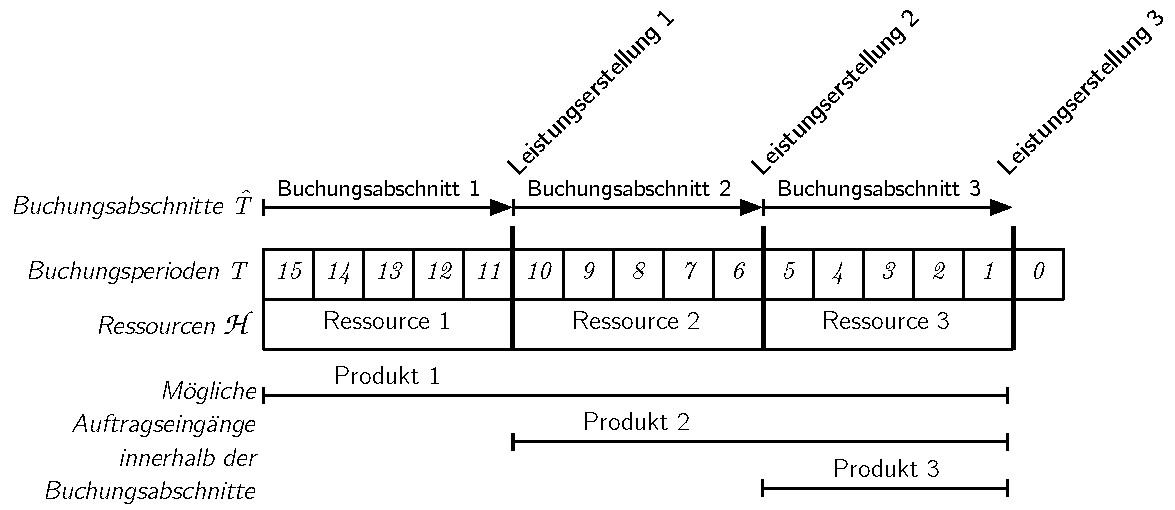
\includegraphics[width=130mm]{Bilder/Leistungsperioden.pdf}
    \caption{Zusammenhand von Buchungsperioden und den Buchungsabschnitten}  \label{IH}
    {\footnotesize \textbf{In Anlehnung an:} ????} 
  \end{center}
\end{figure}

Weiter gibt es die Möglichkeit der Transformation der Ressourcenkapazität hin zu einem Lagerbestand. Der Parameter $y^{\bar{t}}$ dient hier als Lagerbestand für die unterschiedlichen Buchungsabschnitte $\bar{t}\in\bar{T}$. Die Transformation bzw. Instandhaltung erfolgt weiterhin aufgrund des Parameters $a_j$. Es wird damit unterstellt, dass anstelle der Auftragsannahme eines Produkts $j$ die Kapazität der Ressource Verwendung finden den Lagerbestand mit den zukünftig geforderten Produkten zu befühlen. Da in dieser Modellformulierung nur von einer Ressource $h^{\bar{t}}$ ausgegangen wird, erfolgt die Bereinigung des Parameters $a_{j}$ um den Index für die Ressource. Für die Modellerweiterung werden jedoch abhängig des aktuell betrachteten Buchungsabschnitts $\bar{t}\in\bar{T}$ unterschiedliche Varianten des Vektors $\textbf{a}_{j}^{\bar{t}}$ für die Produktanfragen $j\in\mathcal{J}$ benötigt. Dies resultiert aus dem Sachverhalt, dass der Vektor $\textbf{a}_{j}^{\bar{t}}$ nur einen Eintrag für den benötigen Ressourcenverbrauch der Produktanfrage $j\in\mathcal{J}$ besitzt und dieser abhängig des Buchungsabschnitts $\bar{t}\in\bar{T}$ wechselt. Existieren zum Beispiel zwei Buchungsabschnitte $\bar{t}$ und beläuft sich der Ressourcenverbauch $a_j$ einer Produktanfrage $j$ auf 2 Einheiten, dann kann die Reduktion der Kapazitäten $c^{\bar{t}}_{h^{\bar{t}}}$ zu den jeweiligen Buchungsabschnitten $\bar{t}\in\bar{T}$ erfolgen. Es existieren damit zwei Vektoren für den Ressourcenverbrauch für die Produktanfrage: ${\textbf{a}_{j}^{\bar{t}}}^{\textbf{T}}=\{ (2,0), (0,2)\}$.

Aufgrund der bisherigen Modellformulierung wird die Modifizierung der Menge an möglichen Ausführungsmodi $\textbf{m}\in\mathcal{M}_{j}$ benötigt. Die Ressource $h^{\bar{t}}$ ist speziell für die jeweilige Leistungsperiode $\bar{t}\in \bar{T}$ vorgesehen und daher kann eine Transformation der Ressource $h^{\bar{t}}$ aus der aktuellen Leistungsperiode $\hat{t}$ nur zu der aktuellen und zu den nächstfolgenden Leistungsperioden $\bar{t}\in \bar{T}$ erfolgen. Sei der Parameter $\tilde{\bar t}$ alle möglichen nachfolgenden Buchungsabschnitte des Buchungsabschnitts $\bar{t}$, dann ist die Menge aller möglichen Ausführungsmodi $\mathcal{M}_{j}^{\tilde{\bar t}\ge \bar{t}}\subseteq\mathcal{M}_j$. Die Menge wird im nachfolgenden als $\mathcal{M}_{j}^{+}$ bezeichnet. Damit existieren zum Beispiel für die Anfrage nach $j$ aufgrund des Ressourcenverbrauchs $\textbf{a}_{j}^{\bar{t}}=(0,2,0,0)$ die Ausführungsmodi $\mathcal{M}_{j}^{+}$: $\{ (0 ,2, 0, 0), (0, 1, 1, 0), (0, 1, 0, 1),$ $(0, 0, 2, 0),$ $(0, 0, 1, 1), (0, 0, 0, 2)\}$. 

Die \textit{Bellman'schen Funktionsgleichung} für die Inanspruchnahme der Kapazitäten zur Aufstockung eines Lagerbestands für nachfolgende Produktanfragen definiert sich damit wie folgt:
\begin{equation}\label{time}
\begin{alignat*}{2}
V(\textbf{c}^{\bar{t}}, \textbf{y}^{\bar{t}}, t) = \;& V(\textbf{c}^{\bar{t}}, \textbf{y}^{\bar{t}}, t-1)+ \sum_{j \in \mathcal{J}}p_{j}(t)[\max[r_{j} - V(\textbf{c}^{\bar{t}}, \textbf{y}^{\bar{t}}, t-1)\\
&+ V(\textbf{c}^{\bar{t}}-\textbf{a}^{\bar{t}}_j, \textbf{y}^{\bar{t}}, t-1),0] \\
&+ \max[r_{j} - V(\textbf{c}^{\bar{t}}, \textbf{y}^{\bar{t}}, t-1) + V(\textbf{c}^{\bar{t}}, \textbf{y}^{\bar{t}}-\textbf{a}_j^{\bar{t}}, t-1),0]\\
&+ \max_{\textbf{m}\in\mathcal{M}_{j}^{+}}[V(\textbf{c}^{\bar{t}}-\textbf{a}^{\bar{t}}_j, \textbf{y}^{\bar{t}}+\textbf{m}, t-1) - V(\textbf{c}^{\bar{t}}, \textbf{y}^{\bar{t}}, t-1) ,0]]\\
\end{alignat*}
\end{equation}


Zur Veranschaulichung der Modellerweiterung wird ein Beispiel eingeführt:

\begin{center}
$j = \{1, 2, 3\}, \; h^{\bar{t}} = \{1\}, \; r_{1} = 100, \; r_{2} = 200, \; r_{3} = 5000,$ \\
$\text{Startperiode } t=3, \; \bar{T}= \{1: \{3\},\; 2: \{2\},\;3: \{1\} \} $,
\end{center}
\[
    \textbf{c}^{\bar{t}}=\begin{pmatrix} 1\\ 1\\ 1  \end{pmatrix}, \;
    a_{1}=1, \;
     a_{2}=1, \;
       a_{3}=2, \;
            p_{j}(t)=
       \begin{pmatrix}
       0.3 & 0.3 & 0.3 \\
0 & 0.3 & 0.3 \\
0 & 0 & 0.3
\end{pmatrix}, 
  \]
  \[
    \textbf{y}^{\bar{t}}= \begin{pmatrix} 0\\ 0\\ 0  \end{pmatrix}, \;
    \textbf{y}^{\bar{t},max}=\begin{pmatrix} 0\\ 0\\ 2  \end{pmatrix}
      \]

Bei dem Beispiel handelt es sich um ein RM Netzwerk mit den vorausgegangen Modellannahmen. Eine Ressource $h^{\bar{t}}$ über alle Perioden $T$. Dabei nimmt die Ressource $h^{\bar{t}}$ zu jedem Buchungsabschnitt $\bar{t}$ den vordefinierten Kapazitätswert $c^{\bar{t}}_{h^{\bar{t}}}$ an. Zur Vereinfachung des Beispiels kann eine Instandhaltung nur zum letzten Buchungsabschnitt erfolgen. Dieses wird gesteuert durch den Parameter $\textbf{y}^{\bar{t},max}$. Aufgrund der Werte der Parameter ergeben sich der in Abbildung \ref{B8} gezeigten Systemzustände und die Erwartungswerte aus der Tabelle \ref{Tab8}.

\begin{figure}[h!]
  \begin{center}
    \includegraphics[width=200mm, angle=90]{Bilder/Beispiel8.pdf}
    \caption{Darstellung der Systemzustände des Netzwerk RM mit Inanspruchnahme von Kapazität zur Aufstockung eines Lagerbestands für nachfolgende Produktanfragen}  \label{B8}
    {\footnotesize \textbf{Legende:} Die Zahlen stehen für den Produktauftrag $j$, AA='Auftragsannahme', LE='Lagerentnahme', IH='Instandhaltung', KA='Kein Auftrag', $\cdots$='Anfrage ablehnen'} 
  \end{center}
\end{figure}

\begin{table}
\begin{footnotesize}
    \caption{Ergebnistabelle für das beispielhafte Netzwerk RM mit der Inanspruchnahme der Kapazitäten zur Aufstockung eines Lagerbestands für nachfolgende Produktanfragen} \label{Tab8}
    \vspace*{3mm}
    \begin{center}
\csvautotabular{data/beispiel8.csv}
      \end{center}
    \begin{center}
          {\footnotesize \textbf{Legende:} AA='Auftragsannahme', LE='Lagerentnahme', IH='Instandhaltung', KA='Kein Auftrag'} 
      \end{center}
\end{footnotesize}
\end{table}

Da es sich hier um Parameter handelt, die in Abhängigkeit des Buchungsabschnitts $\bar{t}$ stehen, wird ein Systemzustand im Netzwerk als Zahlenfolge $[c^1,c^2,c^3,y^1,y^2,y^3,t]$ definiert. Dabei beschreibt der hochgestellt Index den Buchungsabschnitt $\bar{t}\in\bar{T}$. Der beste Pfad für dieses Netzwerk lautet $[1\;1\;1\;0\;0\;0\;3] \rightarrow_{j_{IH}=1[0\;0\;1]} [0\;1\;1\;0\;0\;1\;2] \rightarrow_{j_{IH}=1[0\;0\;1]}  [0\;0\;1\;0\;0\;2\;1]  \rightarrow_{j_{LE}=3} [0\;0\;1\;0\;0\;0\;0]$. Die optimale Politik im Netzwerk besteht aus der Annahme aller Produktanfragen, sofern diese im Systemzustand möglich sind (Vgl. Abbildung \ref{B8}). Innerhalb der ersten zwei Buchungsabschnitte ist der beste Auftragseinfang eine Instandhaltung (IH) im einzig möglichen Moduls $\textbf{m}=(0,0,1)$. Dadurch entsteht ein Lagerbestand, der zur Annahme einer Produktanfrage $j=3$ im Buchungsabschnitt $\bar{t}=3$ Verwendung findet. Dieses Beispiel soll in Abbildung \ref{B8} hauptsächlich die möglichen Optionen bzw. Entscheidungsalternativen für die möglichen Systemzuständen verdeutlichen. Die eigentliche Funktionsweise der Modellerweiterung geht verloren, da die Anzahl an Buchungsperioden $t\in T$ der Anzahl der möglichen Buchungsabschnitte $\bar{t}\in\bar{T}$ entspricht. Zur besseren Veranschaulichung wird ein umfangreicheres Beispiel berechnet.
\begin{center}
$j = \{1, 2\}, \; h^{\bar{t}} = \{1\}, \; r_{1} = 100, \; r_{2} = 5000,$ \\
$\text{Startperiode } t=10, \; \bar{T}= \{1: \{10,9,8,7,6\},\; 2: \{5,4,3,2,1\}\}  $,
\[\textbf{c}^{\bar{t}}=\begin{pmatrix} 1\\ 1  \end{pmatrix}, \;
    a_{1}=1, \;
       a_{2}=2,   \]
         \[ p_{j}(t)=
       \begin{pmatrix}
       0.3 & 0.3 & 0.3 & 0.3 & 0.3 & 0.3 & 0.3 & 0.3 & 0.3 & 0.3\\
0 & 0 & 0 & 0 & 0 & 0.3 & 0.3 & 0.3 & 0.3 & 0.3
\end{pmatrix}, 
  \]
  \[
    \textbf{y}^{\bar{t}}= \begin{pmatrix} 0\\ 0\end{pmatrix}, \;
    \textbf{y}^{\bar{t},max}=\begin{pmatrix} 1\\ 2  \end{pmatrix}
      \]
\end{center}

\begin{table}
\begin{footnotesize}
    \caption{Optimale Politik für das zweite beispielhafte Netzwerk RM mit der Inanspruchnahme der Kapazitäten zur Aufstockung eines Lagerbestands für nachfolgende Produktanfragen} \label{Tab9}
    \vspace*{3mm}
        \begin{center}
\csvautotabular{data/beispiel9a.csv}
      \end{center}
    \begin{center}
      {\footnotesize \textbf{Legende:} AA='Auftragsannahme', LE='Lagerentnahme', IH='Instandhaltung', KA='Kein Auftrag'} 
      \end{center}
\end{footnotesize}
\end{table}

Aufgrund des Umfangs des Buchungshorizonts ist die grafische Darstellung der Systemzustände für dieses Beispiel nicht mehr zielführend, daher wird darauf verzichtet. Tabelle \ref{Tab9} zeigt die ermittelten Erwartungswerte inkl. der optimalen Politik. Tabelle \ref{Erg9} zeigt für eine strategische Entscheidung den besten Pfad der Auftragseingänge.

\begin{table}
\begin{footnotesize}
    \caption{Bester Pfad für das zweite beispielhafte Netzwerk RM mit der Inanspruchnahme der Kapazitäten zur Aufstockung eines Lagerbestands für nachfolgende Produktanfragen} \label{Erg9}
    \vspace*{3mm}
        \begin{center}
\csvautotabular{data/ergebnis9.csv}
      \end{center}
    \begin{center}
      {\footnotesize \textbf{Legende:} LE='Lagerentnahme', IH='Instandhaltung', KA='Kein Auftrag'} 
      \end{center}
\end{footnotesize}
\end{table}

Aufgrund des umfangreichen Buchungshorizonts ist die optimale Politik des Beispiels anfangs keine Anfragen anzunehmen. Erst zur Periode $t=7$ verändern sich die OK insofern, dass der potentielle Ertrag eine Annahme einer Produktanfrage $j\in\mathcal{J}$ rechtfertigt. Jedoch ist zum Zeitpunkt $t=7$ die Instandhaltung (IH) die optimale Politik. Zum nächsten Zeitpunkt $t=6$ kann keine Anfrage angenommen werden, da keine Kapazitäten $c^{\bar{t}}_{h^{\bar t}}$ für den aktuellen Buchungsabschnitt $\bar{t}=1$ verfügbar sind. Erst mit Übergang vom Zeitpunkt $t=5$ zu $t=6$ erfolgt der Wechsel in den nächsten Buchungsabschnitt $\bar{t}=2$. Damit ist wieder eine Einheit der Ressourcenkapazität $c^{\bar{t}}_{h^{\bar{t}}}$ vorhanden. Die optimale Politik für das Unternehmen zum Zeitpunkt $t=5$ ist demnach die weitere Instandhaltung der Ressource $h^{\bar{t}}$ hin zum Lagerbestand $y^{\bar{t}}$ zum Buchungsabschnitt $\bar{t}=2$. Durch diese Politik ist zum Zeitpunkt $t=4$ eine Lagerentnahme (LE) des Produkts $j=2$ möglich, was die Annahme dieser Produktanfrage entspricht. Dadurch wird ein Ertrag in Höhe von $5000$ GE generiert.